\section{Closed-loop Model Checking Using the Abstraction Tree}
After the abstraction tree is built, it can be used for closed-loop model checking. The next question is how to navigate through the abstraction tree so that the most appropriate model(s) are selected for different requirements, and provide the most concrete counter-examples, possibly under multiple physiological conditions, for the physicians to determine the validity of the counter-examples. \cite{uppaal}
\subsection{Select Initial Abstraction(s) Appropriate For the Requirement}
Physiological requirements are in general conditional in the sense that they require conditions to hold under certain open-loop physiological constraints. These constraints map to parameters for certain transitions of the physiological models, which may be merged during the abstraction process.
The most abstract model in the abstraction tree is built to cover the input space to the device as much as possible, thus it may not have enough details to constrain the behaviors of the model according to the constraints in the requirement. Thus the first step of closed-loop model checking is to select the most abstract models which are appropriate for the requirement. A model $M$ is appropriate for a requirement $Req$ if the environment transitions mentioned in the requirement, denoted as $EnvT(Req)$, is a subset of the environment transitions associated with the model $EnvT(M$). The following algorithm finds the most abstract heart models in the abstraction tree $HM\_tree$ that are appropriate for a requirement $Req$.
\begin{Verbatim}
Algorithm 1
function [HM]=eligible(HM_tree,Req)
BM = root of HM_tree
while (BM is not empty)
 For every model M in BM
  If (EnvT(M) \cap EnvT(Req) == EnvT(Req))
   Remove M from BM
   save M in HM
  else
   add children of M in BM
  endif
 endfor
endwhile
Return HM
\end{Verbatim}
%BM = all models in HM_tree with all Prop(Req)
%For all M in BM
 %while (in the parent of M no behavior in Prop(Req) is abstracted with other behaviors)
	 %M = parent of M
 %endwhile
 %save M in HM
 %endfor
\subsection{Obtaining Concrete Counter-examples Under Corresponding Physiological Conditions}
One challenge for modeling physiological environment of medical devices is the large variety of physiological conditions that the devices may encounter. %It is impossible to exhaustively model the conditions with concrete physiological models. 
The set of concrete models (the leave nodes in the abstraction tree) only represent a subset of all possible physiological conditions, thus model checking the device on all of the concrete models is not enough to guarantee the satisfaction of the requirement. By applying physiological abstraction rules, additional physiological-relevant behaviors are incorporated into the abstract models by over-approximation, providing more coverage. 
However, if model checking on an abstract model returns a counter-example, if is difficult to determine whether the counter-example is a valid execution. Due to the incomplete nature of the set of concrete models, if the counter-example cannot be concretized on all the concrete models, it does not mean it is invalid. Therefore it is up to the physician to decide whether a counter-example is valid or not. The algorithm below explore the abstraction tree during model checking and provide the physician the most concrete counter-example(s), if there exists any. 
\begin{Verbatim}
Algorithm 2
Input: system model PM, abstraction tree for environment HM_tree, requirement Req
Output: Counter examples CE and corresponding model refinements
[HM]=eligible(HM_tree,Req);
Mc= HM;
 while (Mc is not empty)
  For all M in Mc
   [satisfied,CE]=ModelChecking(M,PM,Req);
	 Remove M from Mc
	 If satisfied==0
	  add the children of M to Mc
		cache CE
	else
		save CE from the parent model
	endif
 endfor
endwhile
Return all saved CEs and their corresponding models
\end{Verbatim}

\section{Case Study: Closed-loop Model Checking of a Dual Chamber Pacemaker}
\subsection{Pacemaker Model}
\begin{figure}[!t]
		\centering
		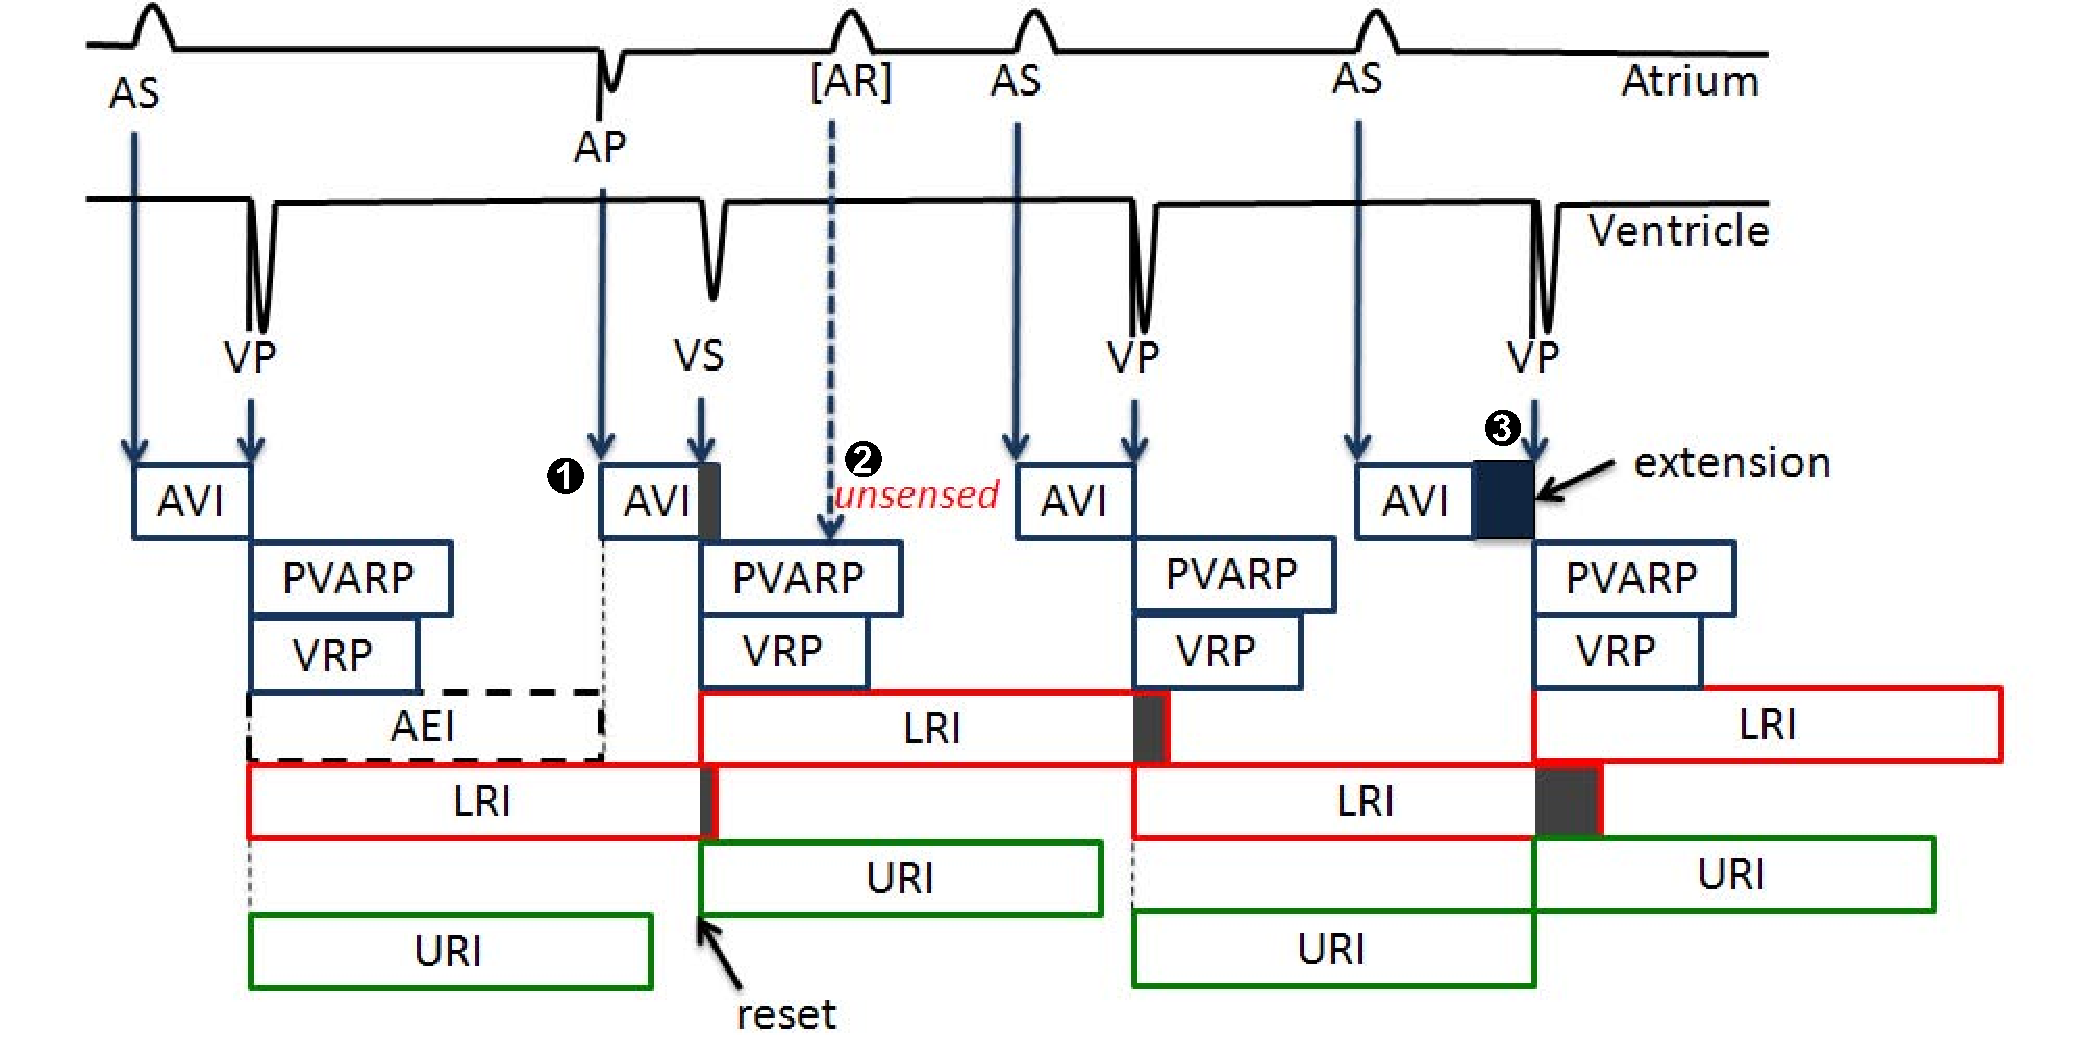
\includegraphics[width=0.5\textwidth]{figs/PM_timers.pdf}
		%\vspace{-5pt}
		\caption{\small Heart Model Abstractions}
		  %\vspace{-15pt}
		\label{fig:PM_timers}
\end{figure}

\subsection{Requirement Encoding}
Physiological requirements can be automatically mapped to model behaviors and parameters. In general, a requirement has \emph{pre-conditions} under which the requirement should hold. The pre-conditions are open-loop physiological conditions which are in terms of constraints on model behaviors. The \emph{post-conditions} are closed-loop behaviors that the device should achieve. The requirement below is designed to prevent the pacemaker from pacing too fast.
\begin{itemize}
	\item Pre-condition: Atrial self-activation rate (60bpm - 200bpm)
    \item Post-condition: Intervals between ventricular paces should be no shorter than 500ms
\end{itemize}

With behavior mapping and a monitor (\figref{monitor}), the requirement can be translated to:
$$Req1: NA.self.min=300 \&\& NA.self.max=1000 \Rightarrow not M.Err$$
The environment behavior specified in $Req1$ is $EnvB(Req1)=NA.self$.
\subsection{Choosing Appropriate Heart Model For the Requirement}
To verify the closed-loop system with pacemaker model $PM$ and heart model abstraction tree $HM\_tree$ (\figref{abs_exam}) against requirement $Req1$, we start by searching for the most abstract appropriate models from the abstraction tree. We call the function specified in Algorithm 1: $[HM]=eligible(HM\_tree,Req1)$. At the root level heart model $H_{all}$, $NA.self$ is abstracted with $(NA',NV').cond$. As the result, $H_{all}$ is not appropriate for $Req1$. $NA.self$ is not abstracted with other behaviors in the children of $H_{all}$: $H_n'',H_{at}'''',H_{vt}'''$, thus these 3 heart models are outputted as the most abstract appropriate models for $Req1$.
\subsection{Providing Meaningful Counter-examples to the Physicians}
After we choose the appropriate models for $Req1$, we have: 
$$HM=\{H_n'',H_{at}'''',H_{vt}'''\}$$
Then we run Algorithm 2. By model checking on all 3 initial models in UPPAAL we have: 
$$[1,[]]=ModelChecking(H_n'',PM,Req1)$$
 $$[0,CE_1]=ModelChecking(H_{at}'''',PM,Req1)$$
$$[0,CE_2]=ModelChecking(H_{vt}''',PM,Req1)$$
The algorithm keeps going down the abstraction tree, and at certain intermediate step we have:
 $$[0,CE_a]=ModelChecking(H_{st}',PM,Req1)$$
  $$[0,CE_b]=ModelChecking(H_{pvc}',PM,Req1)$$
	$$[0,CE_c]=ModelChecking(H_{at},PM,Req1)$$
 $$[1,[]]=ModelChecking(H_{vr}'',PM,Req1)$$
 $$[1,[]]=ModelChecking(H_{vf}'',PM,Req1)$$

\begin{figure}[!t]
		\centering
		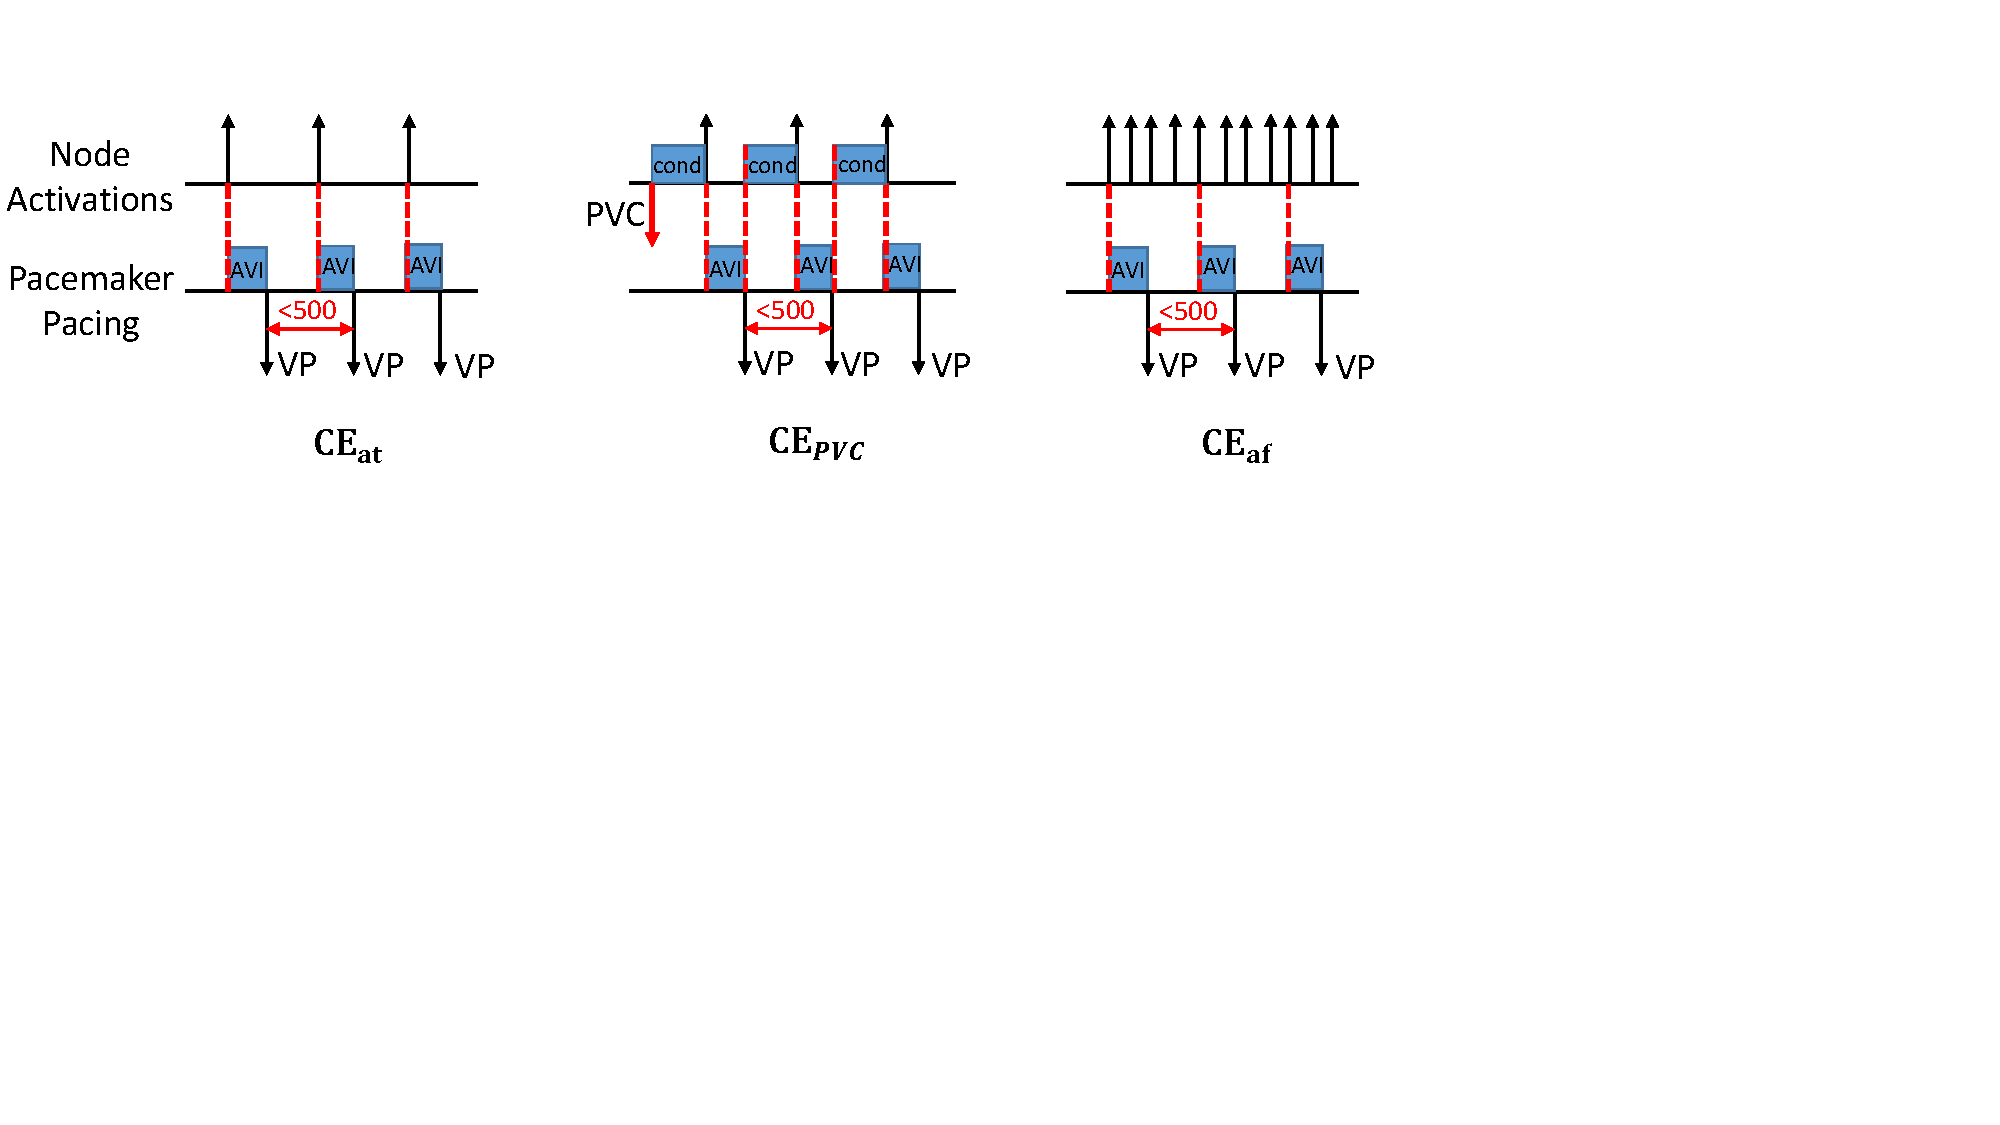
\includegraphics[width=0.9\textwidth]{figs/case.pdf}
		%\vspace{-5pt}
		\caption{\small Counter-examples}
		  %\vspace{-15pt}
		\label{fig:CE}
\end{figure}
The counter-examples from more refined models provide more detailed mechanism of the requirement violations, and distinguish the physiological conditions that can trigger the violations. It is much easier for the physician to determine the validity of the counter-example. The counter-examples from the example above are illustrated in \figref{CE}. $CE_a$ corresponds to fast intrinsic heart rate thus is a safe execution of the pacemaker. $CE_b$ corresponds to a scenario called Endless Loop Tachycardia during which the pacemaker and the heart forms a conduction loop that increases the heart rate inappropriately. In $CE_c$ the pacemaker extends fast atrial rate to more dangerous fast ventricular rate, which is referred to as Atrial Tachycardia Response of a pacemaker. Both $CE_b$ and $CE_c$ are inappropriate executions of the pacemaker .$CE_a$ and $CE_b$ can have the same input-output executions on the pacemaker side and can only be differentiated on the heart model side. After the physician examines the counter-example the programmer can work on debugging.
%$NA\_self$ is in $H_3$, we go one level up, in $H_4$ the behavior is not merged with any other parameters. In $H_5$ $NA\_self$ is merged with  $NA'-NV'.cond$ so $H_4$ is returned as the appropriate heart model for R1. In \cite{STTT13} we used $H_4$ to verify the correctness of the ELT termination algorithm. With a basic DDD pacemaker we have $H_4 || P_{DDD}\models R1$. The counter-example returned is exactly the ELT behavior. Then we implement the ELT termination algorithm and we have  $H_4 || P_{ELT}\not\models R1$, meaning ELT has been successfully terminated, and only the ELT is terminated. 
%
%\subsection{Inappropriate Model Refinements}
%If we follow the traditional CEGAR framework and verify the property using $H_5$, an abstract counter-example would return, which is shown in %\figref{C_amiguity}. However the counter-example correspond
 




